%%%%%%%%%%%%%%%%%%%%%%%%%%%%%%%%%%%%%%%%%
% Wenneker Assignment
% LaTeX Template
% Version 2.0 (12/1/2019)
%
% This template originates from:
% http://www.LaTeXTemplates.com
%
% Authors:
% Vel (vel@LaTeXTemplates.com)
% Frits Wenneker
%
% License:
% CC BY-NC-SA 3.0 (http://creativecommons.org/licenses/by-nc-sa/3.0/)
%
%%%%%%%%%%%%%%%%%%%%%%%%%%%%%%%%%%%%%%%%%

%----------------------------------------------------------------------------------------
%	PACKAGES AND OTHER DOCUMENT CONFIGURATIONS
%----------------------------------------------------------------------------------------

\documentclass[11pt]{scrartcl} % Font size

%%%%%%%%%%%%%%%%%%%%%%%%%%%%%%%%%%%%%%%%%
% Wenneker Assignment
% Structure Specification File
% Version 2.0 (12/1/2019)
%
% This template originates from:
% http://www.LaTeXTemplates.com
%
% Authors:
% Vel (vel@LaTeXTemplates.com)
% Frits Wenneker
%
% License:
% CC BY-NC-SA 3.0 (http://creativecommons.org/licenses/by-nc-sa/3.0/)
%
%%%%%%%%%%%%%%%%%%%%%%%%%%%%%%%%%%%%%%%%%

%----------------------------------------------------------------------------------------
%	PACKAGES AND OTHER DOCUMENT CONFIGURATIONS
%----------------------------------------------------------------------------------------

\usepackage{amsmath, amsfonts, amsthm} % Math packages

\usepackage{listings} % Code listings, with syntax highlighting

\usepackage[english]{babel} % English language hyphenation

\usepackage[xetex]{graphicx}
%\usepackage{graphicx} % Required for inserting images
\graphicspath{{Figures/}{./}} % Specifies where to look for included images (trailing slash required)

\usepackage{booktabs} % Required for better horizontal rules in tables

\numberwithin{equation}{section} % Number equations within sections (i.e. 1.1, 1.2, 2.1, 2.2 instead of 1, 2, 3, 4)
\numberwithin{figure}{section} % Number figures within sections (i.e. 1.1, 1.2, 2.1, 2.2 instead of 1, 2, 3, 4)
\numberwithin{table}{section} % Number tables within sections (i.e. 1.1, 1.2, 2.1, 2.2 instead of 1, 2, 3, 4)

\setlength\parindent{0pt} % Removes all indentation from paragraphs

\usepackage{enumitem} % Required for list customisation
\setlist{noitemsep} % No spacing between list items

%----------------------------------------------------------------------------------------
%	DOCUMENT MARGINS
%----------------------------------------------------------------------------------------

\usepackage{geometry} % Required for adjusting page dimensions and margins

\geometry{
	paper=a4paper, % Paper size, change to letterpaper for US letter size
	top=2.5cm, % Top margin
	bottom=3cm, % Bottom margin
	left=3cm, % Left margin
	right=3cm, % Right margin
	headheight=0.75cm, % Header height
	footskip=1.5cm, % Space from the bottom margin to the baseline of the footer
	headsep=0.75cm, % Space from the top margin to the baseline of the header
	%showframe, % Uncomment to show how the type block is set on the page
}

%----------------------------------------------------------------------------------------
%	FONTS
%----------------------------------------------------------------------------------------

\usepackage[utf8]{inputenc} % Required for inputting international characters
\usepackage[T1]{fontenc} % Use 8-bit encoding

\usepackage{fourier} % Use the Adobe Utopia font for the document

%----------------------------------------------------------------------------------------
%	SECTION TITLES
%----------------------------------------------------------------------------------------

\usepackage{sectsty} % Allows customising section commands

\sectionfont{\vspace{6pt}\centering\normalfont\scshape} % \section{} styling
\subsectionfont{\normalfont\bfseries} % \subsection{} styling
\subsubsectionfont{\normalfont\itshape} % \subsubsection{} styling
\paragraphfont{\normalfont\scshape} % \paragraph{} styling

%----------------------------------------------------------------------------------------
%	HEADERS AND FOOTERS
%----------------------------------------------------------------------------------------

\usepackage{scrlayer-scrpage} % Required for customising headers and footers

\ohead*{} % Right header
\ihead*{} % Left header
\chead*{} % Centre header

\ofoot*{} % Right footer
\ifoot*{} % Left footer
\cfoot*{\pagemark} % Centre footer
 % Include the file specifying the document structure and custom commands
% LaTeX settings for MATLAB code listings
% based on Ted Pavlic's settings in http://links.tedpavlic.com/ascii/homework_new_tex.ascii
\usepackage{listings}
\usepackage[usenames,dvipsnames]{color}

% This is the color used for MATLAB comments below
\definecolor{MyDarkGreen}{rgb}{0.0,0.4,0.0}

% For faster processing, load Matlab syntax for listings
\lstloadlanguages{Matlab}%
\lstset{language=Matlab,                        % Use MATLAB
        frame=single,                           % Single frame around code
        basicstyle=\scriptsize\ttfamily,             % Use small true type font
        keywordstyle=[1]\color{Blue}\bfseries,        % MATLAB functions bold and blue
        keywordstyle=[2]\color{Purple},         % MATLAB function arguments purple
        keywordstyle=[3]\color{Blue}\underbar,  % User functions underlined and blue
        identifierstyle=,                       % Nothing special about identifiers
                                                % Comments small dark green courier
        commentstyle=\usefont{T1}{pcr}{m}{sl}\color{MyDarkGreen}\small,
        stringstyle=\color{Purple},             % Strings are purple
        showstringspaces=false,                 % Don't put marks in string spaces
        tabsize=3,                              % 5 spaces per tab
        %
        %%% Put standard MATLAB functions not included in the default
        %%% language here
        morekeywords={xlim,ylim,var,alpha,factorial,poissrnd,normpdf,normcdf,imresize,double,immse,fspecial,cell2mat,circshift,cell},
        %
        %%% Put MATLAB function parameters here
        morekeywords=[2]{on, off, interp},
        %
        %%% Put user defined functions here
        morekeywords=[3]{FindESS, homework_example},
        %
        morecomment=[l][\color{Blue}]{...},     % Line continuation (...) like blue comment
        numbers=left,                           % Line numbers on left
        firstnumber=1,                          % Line numbers start with line 1
        numberstyle=\tiny\color{Blue},          % Line numbers are blue
        stepnumber=1                            % Line numbers go in steps of 5
        }

% Includes a MATLAB script.
% The first parameter is the label, which also is the name of the script
%   without the .m.
% The second parameter is the optional caption.
\newcommand{\matlabscript}[2]
  {\begin{itemize}\item[]\lstinputlisting[caption=#2,label=#1]{#1.m}\end{itemize}}


\usepackage{fontspec}
\setmainfont{Tinos Nerd Font} %nice font for english and greek

\usepackage{hyperref} %for hyperlinks
\hypersetup{
    colorlinks=true,
    linkcolor=blue,
    filecolor=magenta,
    urlcolor=cyan,
}
%----------------------------------------------------------------------------------------
%	TITLE SECTION
%----------------------------------------------------------------------------------------

\title{
	\normalfont\normalsize
	\textsc{Technical University of Crete, ECE}\\ % Your university, school and/or department name(s)
	\vspace{25pt} % Whitespace
	\rule{\linewidth}{0.5pt}\\ % Thin top horizontal rule
	\vspace{20pt} % Whitespace
	{\Huge Digital Image Processing}\\ % The assignment title

	{\huge Third Lab Report}\\ % The assignment title
	\vspace{12pt} % Whitespace
	\rule{\linewidth}{2pt}\\ % Thick bottom horizontal rule
	\vspace{12pt} % Whitespace
}

\author{\LARGE{Τσιαούσης Χρήστος}\\
		\texttt{2016030017}
		\and
		\LARGE{Πρωτοπαπαδάκης Γιώργος}\\
		\texttt{2016030134}}% Your name

\date{\normalsize\today} % Today's date (\today) or a custom date

\begin{document}

\maketitle % Print the title

%----------------------------------------------------------------------------------------
%	FIGURE EXAMPLE
%----------------------------------------------------------------------------------------

\section{Σκοπός Εργαστηρίου}

\begin{figure}[h] % [h] forces the figure to be output where it is defined in the code (it suppresses floating)
	\centering
	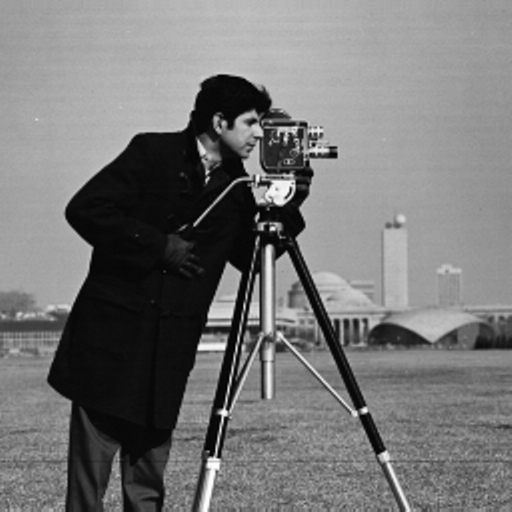
\includegraphics[width=0.5\columnwidth]{cameraman.jpg} % Example image
	\caption{Αρχική εικόνα.}
\end{figure}


Το εργαστήριο έχει ως σκοπό την περεταίρω εξοικείωση μας με την συνέλιξη σε δισδιάστατα σήματα όπως μια grayscale εικόνα καθώς και την αποδοτικότερη
χρήση του matlab και δυνατότητες όπως τα for loops. Καλούμαστε να δημιουργήσουμε decomposition pyramids, δηλαδή την αποσύνθεση των εικόνων. Βλέπουμε
την επαναλημένη εξομάλυνση των edges χρησιμοποιόντας την μεθοδολογία του Gaussian Pyramid, και πως από τα Ν επίπεδα της, μπορεί να δημιουργηθεί η
Laplacian Pyramid όπου τονίζει μόνο τις ακμές στην εικόνα, δηλαδή το αντίστροφο του Gaussian Pyramid. Τέλος βλέπουμε ότι ο συνδυασμός αυτών, μας δίνει
την αρχική εικόνα.
%------------------------------------------------

\section{Gaussian Pyramid}

Για την κατασκευή της Gaussian πυραμίδας, αρχικά, κάνουμε συνέλιξη την αρχική μας εικόνα με gaussian filter \textit{5x5} και standard deviation = 1.
Εισάγουμε το αποτέλεσμα αυτό στο πρώτο επίπεδο \textit{G(0)} της πυραμίδας. Για το επόμενο επίπεδο, κάνουμε down-sample την εικόνα του προηγούμενου
επιπέδου κατά 1/2 και συνελίσουμε ξανά με το ίδιο gaussian filter. Επαναλαμβάνουμε μέχρι να φτάσουμε στο επιθυμητό επίπεδο \textit{G(4)}.


Να σημειωθεί ότι το downsample γίνεται με τις default ρυθμίσεις της συνάρτησης ``imresize''. Θα μπορούσαμε να χρησιμοποιήσουμε μεθοδολογίες από
το πρώτο εργαστήριο για ελαφρώς διαφορετικά αποτελέσματα.


\begin{figure}[h]
    \centering
    \makebox[\textwidth]{\includegraphics[width=\paperwidth]{1.jpg}}
    \caption{Gaussian Pyramid.}
\end{figure}
% \clearpage

\section{Laplacian Pyramid}

Για την κατασκευή της Laplacian πυραμίδας, κάνουμε upsample, διπλασιάζοντας το αμέσως μικρότερο επίπεδο απ την Gaussian Pyramid. Έπειτα αφαιρούμε
το \textit{G(κ)}, όπου κ το επίπεδο που βρισκόμαστε, με το upsampled \textit{G(κ+1)}. Επαναλαμβάνουμε μέχρι να φτάσουμε στο πρότελευταίο επίπεδο
της Gaussian Pyramid.


Ομοίως, με διαφορετικές ρυθμίσεις στο upsample θα μπορούσαμε να καταλήξουμε σε διαφορετικά αποτελέσματα αποσύνθεσης.

\begin{figure}[h]
    \centering
    \makebox[\textwidth]{\includegraphics[width=\paperwidth]{2.jpg}}
    \caption{Laplacian Pyramid.}
\end{figure}
\clearpage

\section{Reconstruction}

Για την ανακατασκευή της εικόνας, απλώς προσθέτουμε ανά επίπεδο τα \textit{G(κ)} και \textit{L(κ)}. Εν τέλει καταλήγουμε με την αρχική εικόνα
και τα διάφορα downsampled επίπεδά της.

\begin{figure}[h]
    \centering
    \makebox[\textwidth]{\includegraphics[width=\paperwidth]{3.jpg}}
    \caption{Reconstruction Pyramid.}
\end{figure}
% \clearpage

% \newpage

\section{Συμπεράσματα}

Οπτικά, το reconstruction γίνεται μια χαρά. Ενδεικτικά, όμως, κοιτάζουμε και τα σφάλματα, συγκρίνοντας το μεγαλύτερο επίπεδο στην Reconstruction Pyramid, με την αρχική εικόνα
καθώς και την αρχική εικόνα συνελιγμένη με το φίλτρο.

\begin{table}[h] % [h] forces the table to be output where it is defined in the code (it suppresses floating)
	\centering % Centre the table
	\begin{tabular}{l c c}
		\toprule
		\textit{σφάλμα} & \textbf{original} & \textbf{convolved} \\
		\midrule
		\midrule
		MSE & 23.50 & 32.34 \\
		\midrule
		PSNR & 34.42 & 33.05 \\
		\bottomrule
	\end{tabular}
	\caption{Τα τελικά σφάλματα.}
\end{table}

Προς έκπληξη μας, η reconstructed εικόνα είναι πιο κοντά στην αρχική απ' ότι στην συνελιγμένη. Η σηματοθορυβική σχέση είναι καλύτερη και το μέσο τετραγωνικό σφάλμα μικρότερο.

Η μεθοδολογία του decomposition έχει ενδιαφέρον και για την ανάλυση μιας εικόνας. Πιο συγκεκριμένα, βλέπουμε ότι μπορούμε να ξεχωρήσουμε τις ακμές από μια εικόνα χρησιμοποιόντας
μόνο ένα φίλτρο. που μάλιστα χρησιμοποιείται για μείωση των ακμών..! Κι επι της ουσίας, χωρίζουμε την φωτογραφία σε περιοχές διαφορετικού και ξεχωριστού μεταξύ τους ενδιαφέροντος
με πολύ μικρές απώλεις. Κι αυτό μπορεί να φανεί από την σύγκριση με την αρχικη εικόνα.


\section{Ο κώδικας που υλοποίησε τα παραπάνω}

\matlabscript {main_3}{Η υλοποίηση σε Matlab}

\matlabscript {padForConv}{Η υλοποίησή μας για τα paddings}

\matlabscript {convolution}{Η υλοποίησή μας για την συνέλιξη}

\end{document}
